\begin{frame}{Инициализация псевдоскоростей на CUDA}

\begin{figure}
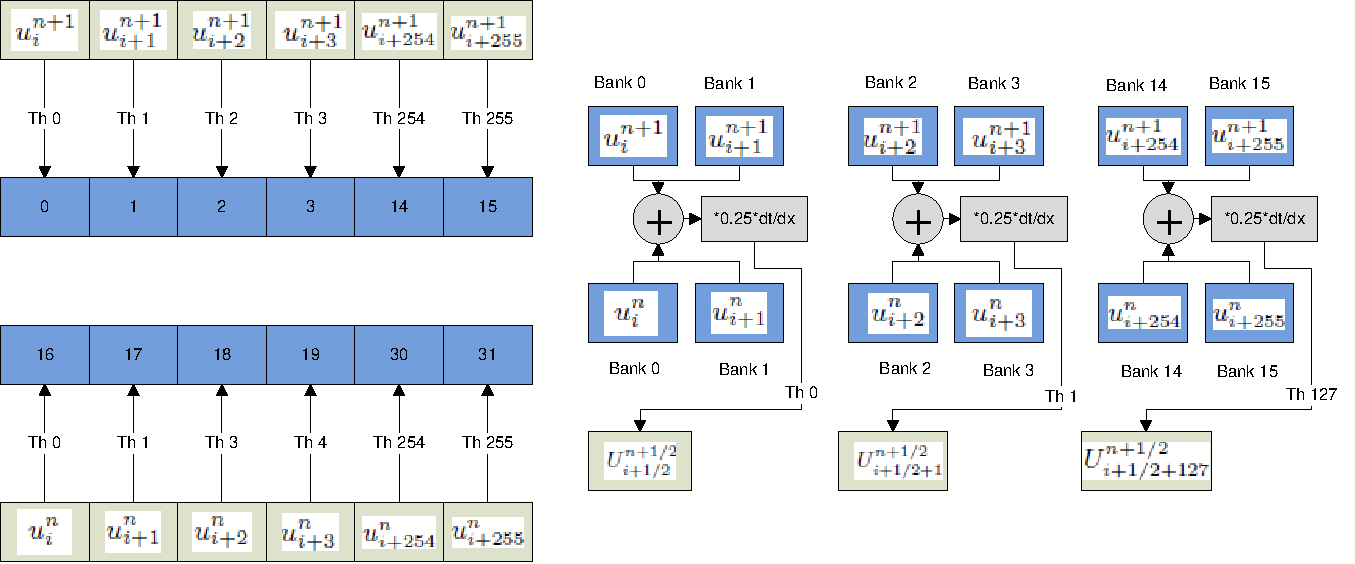
\includegraphics[height=2in, width=3.5in]{artwork/pdf/uu_init}
\label{fig:wrf-equations}
\end{figure}

\[ U^{n+1/2}_{i+1/2}=0.25 \cdot \frac{dt}{dx} \cdot(u^{n-1}_{i-1} + u^{n-1}_{i} + u^{n}_{i-1} + u^{n}_{i}) \]


\begin{itemize}
  \item Склейка по доступу в глобальную память (Coalescing)
  \item Эффективная блокировка варпов (Warps Stall)
  \item Возможен двухкратный конфликт по банкам разд. памяти
\end{itemize}

\end{frame}

\begin{frame}{Анализ производительности мультипроцессора\cite{kirk:cuda}}
\begin{enumerate}
  \item Загрузка $\upsilon^{n+1}_{i+0+..255}$
  \begin{itemize}
        \item $N_{threads}=256 \Rightarrow N_{warps}=\frac{256}{32}=8$ 
        \item $ShMemSize_1 = N_{threads}\cdot 2 \cdot 4 = 2048$ Bytes
  \end {itemize}
  \item Загрузка $\upsilon^{n}_{i+0+..255}$
  \begin{itemize}
        \item $N_{threads}=256 \Rightarrow N_{warps}=\frac{256}{32}=8$
        \item $ShMemSize_2 = N_{threads}\cdot 2 \cdot 4 = 2048$ Bytes
  \end {itemize}
  \item Вычисление $U^{n+1/2}_{i+1/2+..127}$
  \begin{itemize}
        \item $N_{threads}=\frac{256}{2}=128 \Rightarrow N_{warps}=\frac{128}{32}=4$
  \end {itemize}
  \item Анализ загрузки мультипроцессора
  \begin{itemize}
   \item Максимальное количество блоков на мультипроцессоре по потокам $MaxBlocks_{threads}=\frac{1024}{256}=4$
   \item Максимальное количество блоков на мультипроцессоре по разделяемой памяти $MaxBlocks_{shmem}=\frac{MaxShmem}{ShMemSize_1 + ShMemSize_2}=\frac{32768}{2048 + 2048}=8$
  \end {itemize}
  \item Вывод - так как алгоритм memory-bound, то фактором, сдерживающим производительность мультипроцессора, может стать нехватка регистров, если $N_{regs}\gtrdot \frac{16384}{1024}=16$
\end{enumerate}
\end{frame}

